%%%%%%%%%%%%%%%%%%%%%%%%%%%%%%%%%%%%%%%%%%%%%%%%%%%%%%%%%%%%
%%% ELIFE ARTICLE TEMPLATE
%%%%%%%%%%%%%%%%%%%%%%%%%%%%%%%%%%%%%%%%%%%%%%%%%%%%%%%%%%%%
%%% PREAMBLE
\documentclass[9pt,lineno]{elife}
% Use the onehalfspacing option for 1.5 line spacing
% Use the doublespacing option for 2.0 line spacing
% Please note that these options may affect formatting.
% Additionally, the use of the \newcommand function should be limited.

\usepackage{lipsum} % Required to insert dummy text
\usepackage[version=4]{mhchem}
\usepackage{siunitx}
\DeclareSIUnit\Molar{M}

%%%%%%%%%%%%%%%%%%%%%%%%%%%%%%%%%%%%%%%%%%%%%%%%%%%%%%%%%%%%
%%% ARTICLE SETUP
%%%%%%%%%%%%%%%%%%%%%%%%%%%%%%%%%%%%%%%%%%%%%%%%%%%%%%%%%%%%
\title{Effects of delayed strain submission and vaccine development on long-term forecast accuracy of seasonal influenza A/H3N2}

\author[1*]{John Huddleston}
\author[2]{Trevor Bedford}
\affil[1]{Vaccine and Infectious Disease Division, Fred Hutchinson Cancer Center, Seattle, WA, USA}
\affil[2]{Howard Hughes Medical Institute, Seattle, WA, USA}

\corr{jhuddles@fredhutch.org}{JH}

%%%%%%%%%%%%%%%%%%%%%%%%%%%%%%%%%%%%%%%%%%%%%%%%%%%%%%%%%%%%
%%% ARTICLE START
%%%%%%%%%%%%%%%%%%%%%%%%%%%%%%%%%%%%%%%%%%%%%%%%%%%%%%%%%%%%

\begin{document}

\maketitle

\begin{abstract}
TKTK
\end{abstract}

\section{Introduction}

TKTK

\begin{figure}[htb]
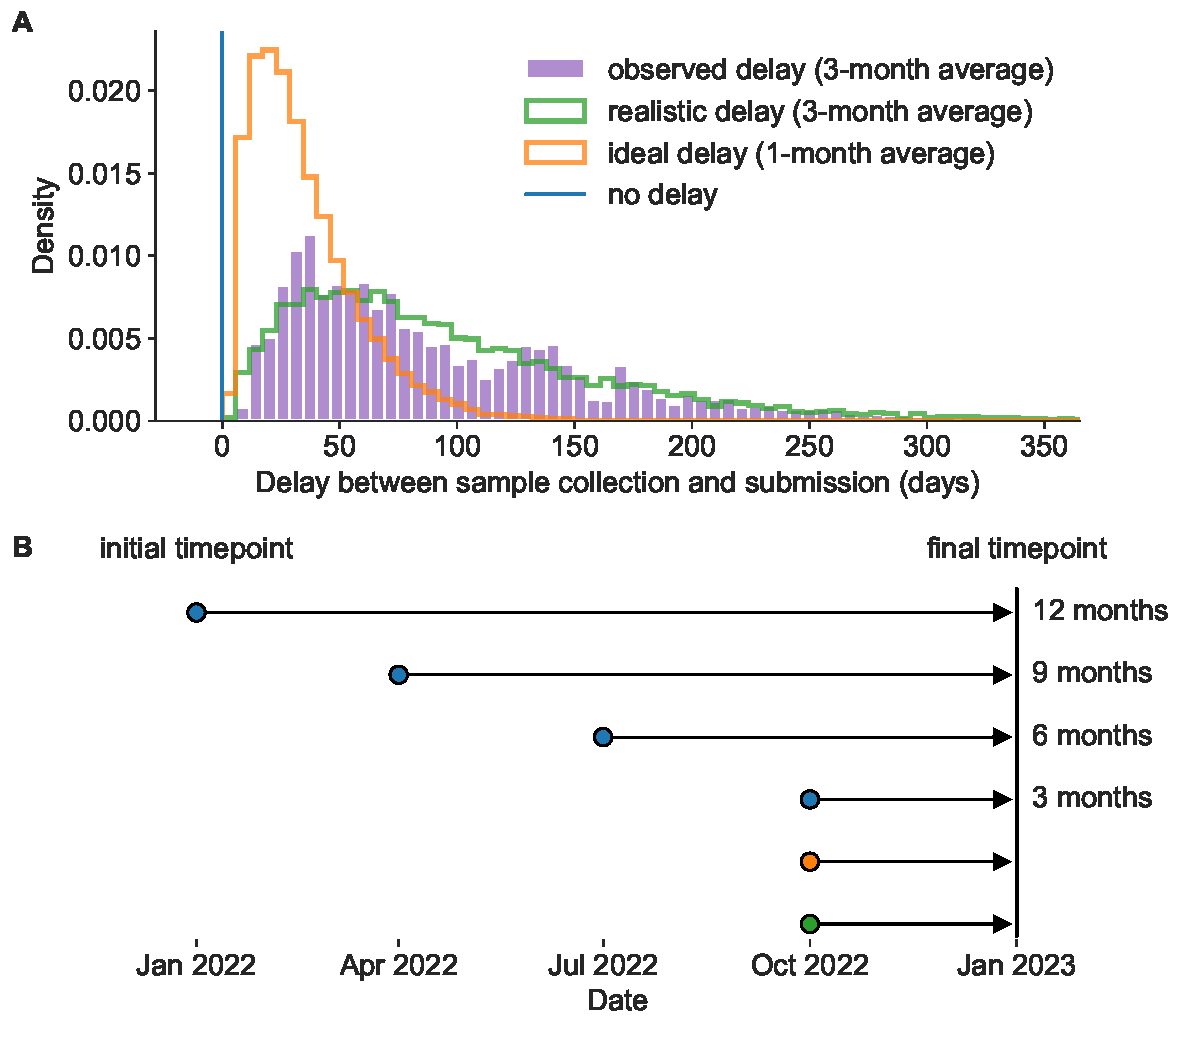
\includegraphics[width=\linewidth]{figures/distribution_of_delays_and_horizons}
\caption{Model of submission delays and forecast horizons.}
\label{fig:model_of_delays_and_horizons}
\end{figure}

\section{Results}

\subsection{Reducing forecast horizons decreases distances between predicted and observed future populations}

Previously, we trained long-term forecasting models that minimized the earth mover's distance \citep{Rubner1998} between predicted and observed future populations \citep{Huddleston2020}.
Each forecast predicted 12 months into the future from a given initial timepoint to a future timepoint.
Specifically, the forecasts predicted the future frequencies of samples circulating at the initial timepoint based on the estimated fitness of each sample.
We calculated the distance between hemagglutinin (HA) amino acid sequences observed at the initial timepoint and the future timepoint, weighting the distance by the predicted future frequency of samples at the initial timepoint and the observed frequency of samples at the future timepoint.
The best forecasting models used fitness estimates that reduced the distance between predicted and observed future populations.
For example, the most accurate sequence-only model for the 12-month forecast horizon estimated fitness with local branching index (LBI) \citep{Neher:2014eu} and mutational load \citep{Luksza:2014hj}.

Here, we produced forecasts 3, 6, 9, and 12 months into the future using HA sequences available at each initial timepoint based on one of three scenarios of delayed sequence submission to public databases: no delay, an ``ideal'' delay ($\sim$1-month average), and a ``realistic'' delay ($\sim$3-month average) (\FIG{model_of_delays_and_horizons}).
For natural A/H3N2 populations, we used the best sequence-only model, LBI and mutational load, which we previously trained on 12-month forecasts without any submission delay.
For simulated A/H3N2-like populations, we used the observed fitness per sample provided by the simulator.
For each forecast horizon and submission delay type, we calculated the earth mover's distance between the predicted future populations under the given delay scenario and the observed future populations without any delay in sequence availability.
We anticipated that reducing either the forecast horizon or the submission delay would reduce the distance to the future in amino acids (AAs), representing increased accuracy of the forecasting models.

As expected, we found that reducing the forecast horizon from the current standard of 12 months linearly reduced the distance to the future population predicted by the LBI and mutational load model (\FIG{h3n2_distances_to_the_future}).
Under the all three submission delay scenarios, the distance to the future reduced by approximately 1 AA on average for each 3-month reduction in forecast horizon (\TABLE{h3n2_distances_to_the_future}).
We observed the greatest average reduction in distance to the future ($\sim$1.4 AAs) between the 6- and 3-month forecast horizons.
Reducing the forecast horizon also noticeably reduced the variance per timepoint in predicted future populations across all delay scenarios (\FIG{h3n2_distances_to_the_future}).
For example, the standard deviation of distances to the future reduced from $\sim$2.6 AAs at the 12-month horizon to $\sim$1 AA at the 3-month horizon (\TABLE{h3n2_distances_to_the_future}).
We observed the same pattern for simulated A/H3N2-like populations (\FIGSUPP[h3n2_distances_to_the_future]{simulated_distances_to_the_future}).
Thus, reducing how far we have to predict into the future increased both forecast accuracy and precision.

In contrast, we found that reducing submission delays from a $\sim$3-month average delay in the realistic scenario to a $\sim$1-month average delay in the ideal scenario had relatively little effect on distance to the future.
At the 12-month forecast horizon, the ideal and realistic delay scenarios produced similar predictions, with the only noticeable improvement observed under the scenario without any submission delays (\FIG{h3n2_distances_to_the_future}).
As the forecast horizon decreased, the effect of submission delays appeared more prominent, with the greatest effect of reduced delays observed at the 3-month forecast horizon.
However, the average improvement from the realistic to the ideal submission delay scenario at the 3-month horizon was still only $~\sim$0.3 AAs (\TABLE{h3n2_distances_to_the_future}).
Reducing submission delays also had little effect on the variance per timepoint in predicted future populations.
Interestingly, we observed a stronger effect of reducing submission delays in simulated A/H3N2-like populations (\FIGSUPP[h3n2_distances_to_the_future]{simulated_distances_to_the_future}).
We found the best average improvement between realistic and ideal delays of $\sim$0.7 AAs at the 3-month horizon.
As with natural A/H3N2 populations, the effect of reducing submission delays appeared to increase as the forecast horizon decreased.
These results indicate that reducing submission delays may have little effect under the current 12-month forecast approach used for influenza vaccine composition, but reducing submission delays could be increasingly important as we forecast from closer to future influenza populations.

\begin{figure}[htb]
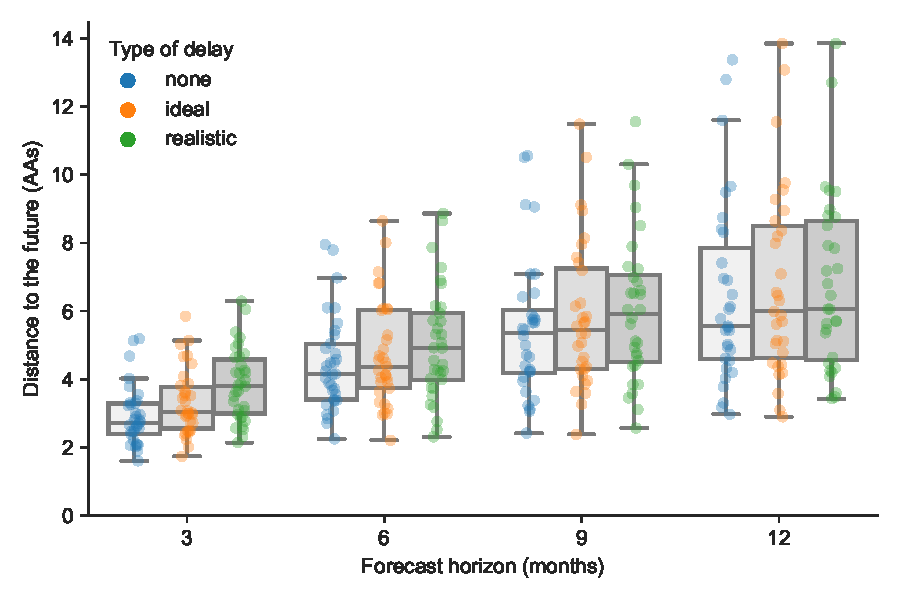
\includegraphics[width=\linewidth]{figures/h3n2_distances_to_the_future_by_delay_and_horizon}
\caption{Distances to the future per timepoint (AAs) for natural A/H3N2 populations by forecast horizon and submission delay type based on forecasts from the local branching index (LBI) and mutational load model.
  Each point represents a future timepoint whose population was predicted from the number of months earlier corresponding to the forecast horizon.
  Points are colored by submission delay type including forecasts made with no delay (blue), an ideal delay (orange), and a realistic delay (green).}
\label{fig:h3n2_distances_to_the_future}
%
\figsupp[Distances to the future for simulated H3N2-like populations]
{Distances to the future per timepoint (AAs) for simulated H3N2-like populations by forecast horizon and submission delay type.
  \figsuppdata{Distances to the future for simulated H3N2-like populations; see \url{https://doi.org/xxx}}}
{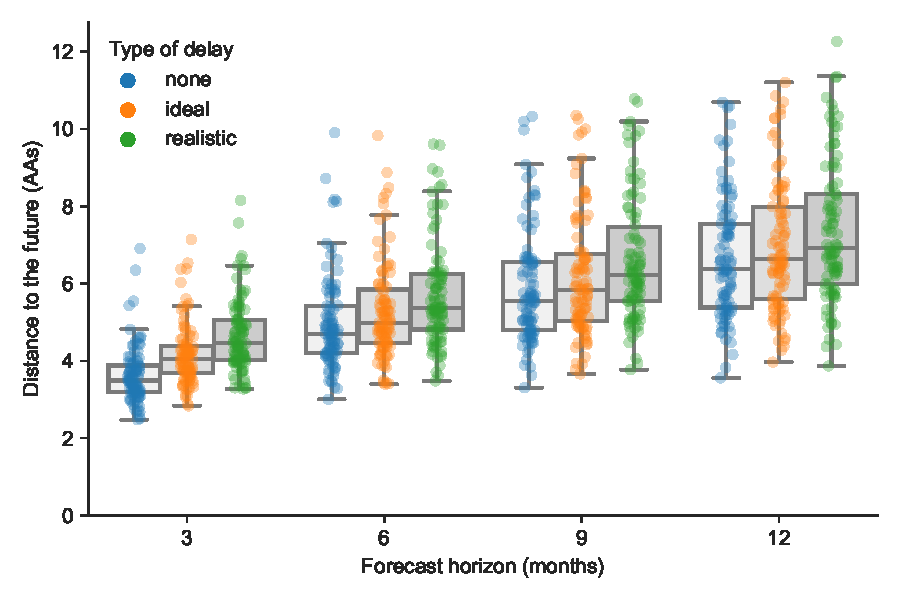
\includegraphics[width=6cm]{figures/simulated_distances_to_the_future_by_delay_and_horizon}}\label{figsupp:simulated_distances_to_the_future}
%
\figdata{Distances to the future for natural H3N2 populations.}\label{figdata:h3n2_distances_to_the_future}
\figsrccode{Jupyter notebook used to produce this figure and the supplemental figure lives in \texttt{workflow/notebooks/plot-distances-to-the-future-by-delay-type-and-horizon-for-population.py.ipynb}.}\label{figsrccode:distances_to_the_future}
\end{figure}

\begin{table}[htb]
  \begin{center}
    
\begin{tabular*}{0.7\textwidth}{rrrr}
\toprule
          & \multicolumn{3}{c}{Distance to future (mean +/- std dev AAs)} \\
  Horizon & No delay & Ideal delay & Realistic delay \\
\midrule

3 & 2.91 +/- 0.86 & 3.32 +/- 0.96 & 3.85 +/- 1.05 \\
6 & 4.44 +/- 1.39 & 4.74 +/- 1.54 & 5.03 +/- 1.66 \\
9 & 5.48 +/- 2.05 & 5.84 +/- 2.14 & 6.04 +/- 2.15 \\
12 & 6.45 +/- 2.72 & 6.77 +/- 2.80 & 6.78 +/- 2.61 \\

\bottomrule
\end{tabular*}


    \caption{Distances to the future in amino acids (mean +/- standard deviation AAs) by forecast horizon (in months) and submission delay for H3N2 populations.}
    \label{tab:h3n2_distances_to_the_future}
  \end{center}
\end{table}

\subsection{Current clade frequency errors}

Although the distance between predicted and observed future populations in amino acids provides an unbiased metric to optimize forecasting models, in practice, we use these models to forecast clade frequencies.
To produce these forecasts, we estimate the frequencies of extant clades at an initial timepoint and predict their future frequencies from those initial frequencies and the fitness estimates of each clade's tips.
Given the importance of initial clade frequencies in these forecasts, we tested the effect of submission delays on current clade frequency estimates.
For each timepoint in our analysis, we summed the frequency per clade assigned to each tip (see Methods).
We calculated the frequency error per timepoint and clade as the difference between the clade frequency without submission delays and the frequency with either an ideal or realistic delay.

\begin{figure}[htb]
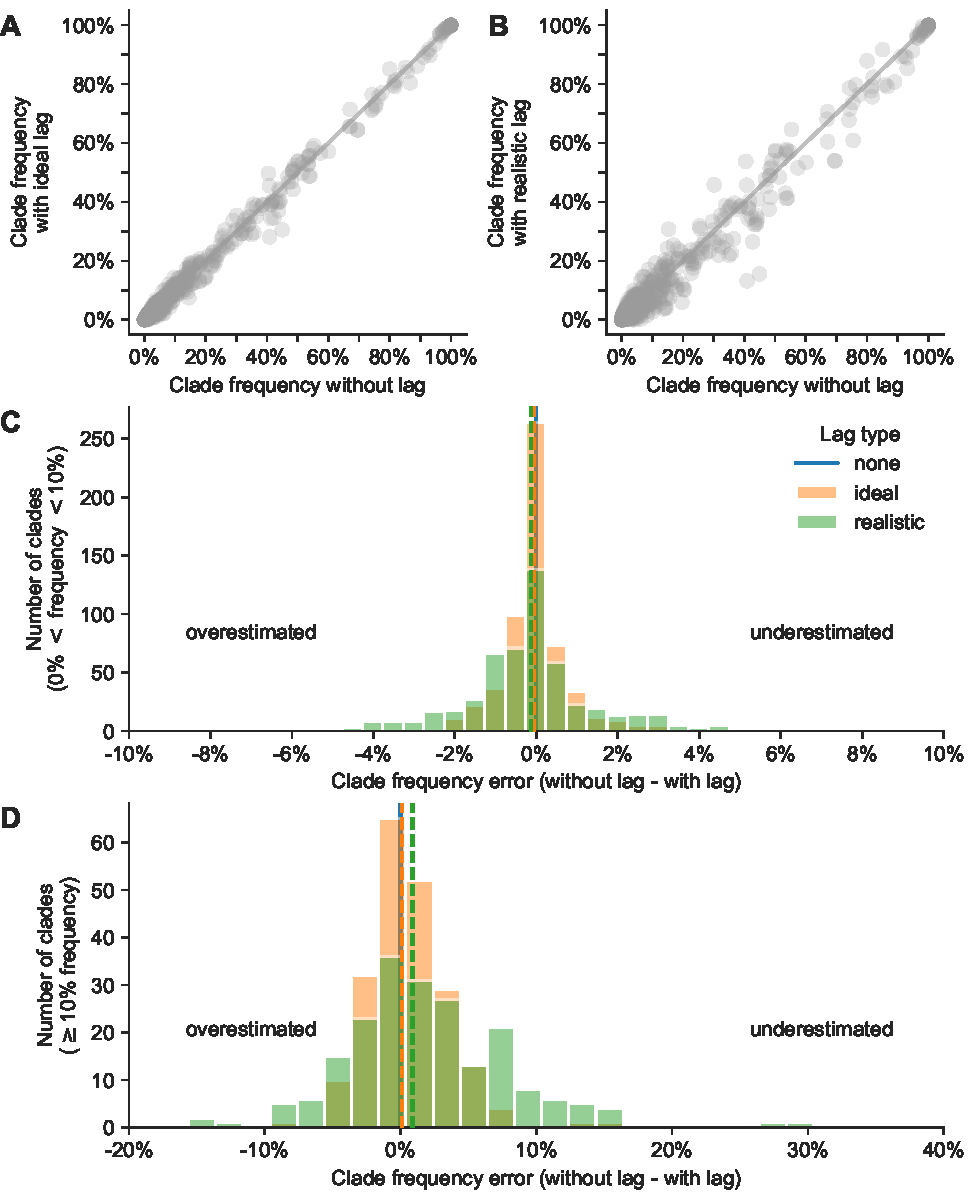
\includegraphics[width=\linewidth]{figures/h3n2_current_frequency_errors_by_delay}
\caption{Clade frequency errors for natural A/H3N2 clades at the same timepoint calculated as the difference between clade frequencies without submission delay and corresponding frequencies with either A) ideal or B) realistic submission delays.
Distributions of frequency errors appear normally distributed in both delay scenarios for both C) small clades ($\ge$1\% and $<$10\% frequency) and D) large clades ($\ge$10\%).}
\label{fig:h3n2_current_clade_frequency_errors}
%
\figsupp[Current clade frequency errors for simulated H3N2-like populations]
{Clade frequency errors between simulated H3N2-like HA populations with ideal or realistic submission delays and populations without any submission delay.
  \figsuppdata{Current frequencies per tip in each simulated H3N2-like tree of the forecast analysis by delay type (none, ideal, and realistic); see \url{https://doi.org/xxx}}}
{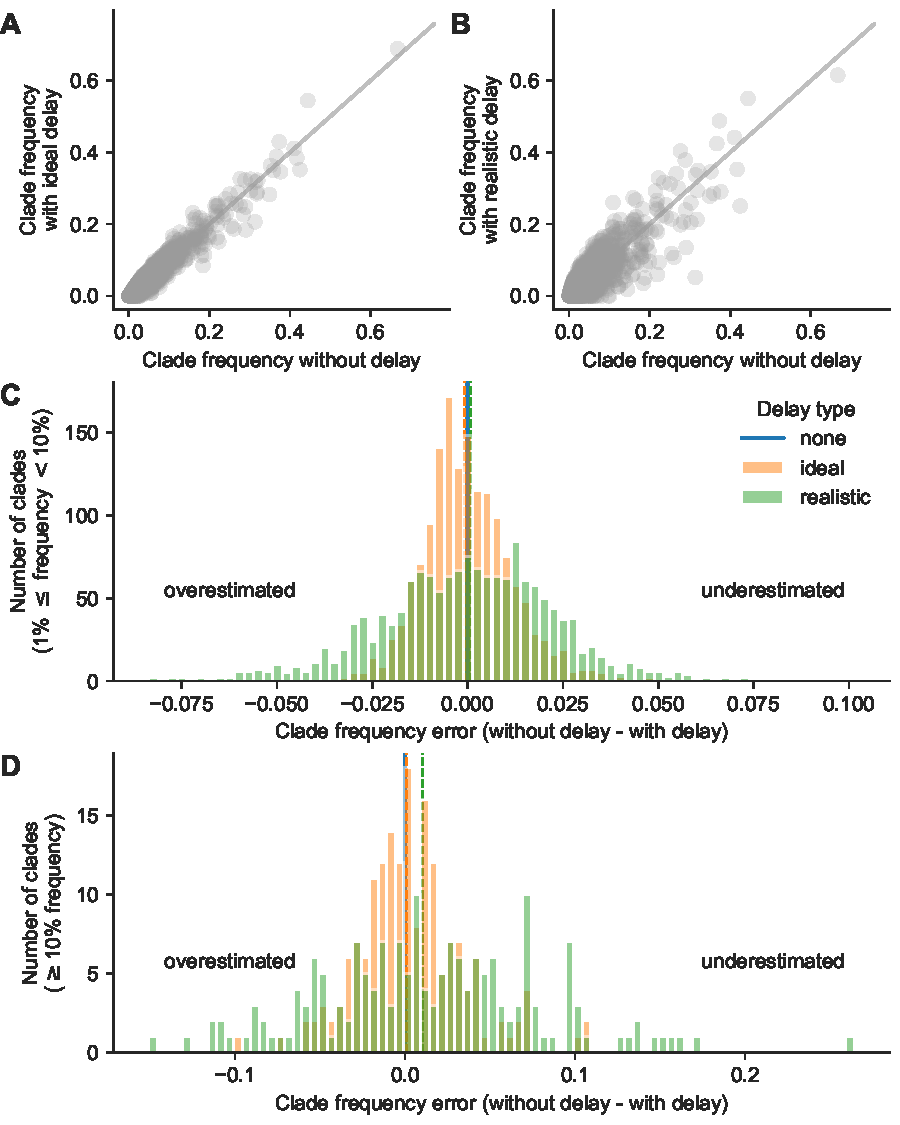
\includegraphics[width=6cm]{figures/simulated_current_frequency_errors_by_delay}}\label{figsupp:simulated_current_clade_frequency_errors}
%
\figdata{Current frequencies per tip in each natural H3N2 tree of the forecast analysis by delay type (none, ideal, and observed).}\label{figdata:h3n2_tip_attributes}
\figsrccode{Jupyter notebook used to produce this figure and the supplemental figure lives in \texttt{workflow/notebooks/plot-current-clade-frequency-errors-by-delay-type-for-populations.py.ipynb}.}\label{figsrccode:current_clade_frequency_errors}
\end{figure}

Surprisingly, we found that even with an average $\sim$1-month delay in submissions, clade frequencies in the ideal delay scenario almost exactly matched frequencies without any delays at all (\FIG{h3n2_current_clade_frequency_errors}A).
For both small clades ($\ge$1\% and $<$10\% frequency without delays) and large clades ($\ge$10\% frequency), clade frequency errors for ideal delays rarely exceeded 1\% (\FIG{h3n2_current_clade_frequency_errors}C and D).
In contrast, realistic delays produced higher errors (\FIG{h3n2_current_clade_frequency_errors}B), ranging between -3\% and 3\% for small clades (\FIG{h3n2_current_clade_frequency_errors}C) and -5\% and 6\% for large clades (\FIG{h3n2_current_clade_frequency_errors}D).
For both delay scenarios, errors appeared normally distributed without a bias toward over- or underestimation of current clade frequencies.
These results indicate that reducing submission delays for influenza sequences from a 3-month to 1-month average could effectively eliminate most of our error in current clade frequency estimates.

Delayed submissions more strongly affected clade frequencies for simulated A/H3N2-like populations (\FIGSUPP[h3n2_current_clade_frequency_errors]{simulated_current_clade_frequency_errors}).
With ideal delays, small clade errors ranged from -5\% to 6\% and large clade errors from -7\% to 13\% (\FIGSUPP[h3n2_current_clade_frequency_errors]{simulated_current_clade_frequency_errors}C and D).
As expected, realistic delays produced higher errors ranging from -13\% to 8\% for small clades and -16\% to 35\% for large clades.
Delays also induced a bias toward underestimation of large clade frequencies with a mean and median error of 1\% with ideal delays and 3\% with realistic delays (\FIGSUPP[h3n2_current_clade_frequency_errors]{simulated_current_clade_frequency_errors}D).
This increased error in frequency estimation for simulated populations corresponds with an overall faster evolutionary rate compared to natural A/H3N2 populations, as we observed in the greater distances to the future for simulated populations (\FIGSUPP[h3n2_distances_to_the_future]{simulated_distances_to_the_future}).
Correspondingly, we would expect seasonal influenza lineages that evolve slower than A/H3N2 (A/H1N1pdm and B/Victoria) to have lower errors in current clade frequency estimates as a result of submission delays.

\subsection{Forecast clade frequency errors}

We estimated the effects of submission delays and forecast horizons on the accuracy of clade frequency forecasts.
For each combination of initial timepoint, future timepoint, and delay scenario (\FIG{model_of_delays_and_horizons}B), we identified all clades that were present at both timepoints, calculated initial and predicted future frequencies for the given delay, and calculated the corresponding observed future frequencies without delay.
Where the current clade frequency analysis focused on the most derived clades assigned to each tip, this analysis included ancestral clades to allow comparison between temporally distant populations.
Therefore, we focused this analysis on clades with an initial frequency $\ge$10\% and $\le$95\% in the corresponding dataset without delays.
We calculated the error in forecast frequencies for these clades as the difference between predicted future frequencies under the given delay scenario and observed future frequencies without any delay.

As with current clade frequency errors, forecast clade frequency errors appeared to be normally distributed with mean and median errors near zero and relatively variance (\FIG{h3n2_forecast_clade_frequency_errors}).
The 12-month forecast horizon produced the most extreme average forecast error (-3\% to -4\%) and standard deviation in error (30\% to 33\%) with a slight bias toward overestimation of future clade frequencies in all delay scenarios (\TABLE{h3n2_forecast_clade_frequency_errors}).
As the forecast horizon decreased, the average error shifted toward 1\% at the 3-month horizon, representing a slight underestimation of future frequencies.
The variance in forecast error also decreased with decreasing horizon, following the same pattern we observed for distances to the future.
In the realistic delay scenario, the standard deviation in forecast error decreased an average of 7\% with each 3-month decrease in forecast horizon from a maximum of 33\% at the 12-month horizon to a minimum of 11\% at the 3-month horizon.
Correspondingly, we observed a wide range of forecast errors at the 12-month horizon and realistic delay spanning from nearly -100\% to over 75\% error.
At the 3-month horizon, errors rarely exceeded 25\% in either direction.

As we observed with distances to the future, reducing submission delays had little effect on the accuracy of clade frequency forecasts.
The mean and median clade frequency errors were almost identical across all delay types (\TABLE{h3n2_forecast_clade_frequency_errors}).
The same pattern held for absolute clade frequency errors (\FIGSUPP[h3n2_forecast_clade_frequency_errors]{h3n2_absolute_forecast_clade_frequency_errors}, \TABLE{h3n2_absolute_forecast_clade_frequency_errors}).
These results suggest that the magnitude of errors caused by increased forecast horizon and bias in the forecasting model negate the benefits of reducing current clade frequency errors by reducing submission delays.

Compared to natural H3N2 populations, forecast errors for simulated A/H3N2-like populations exhibited a stronger tendency toward underestimation across all horizons and delays (\FIGSUPP[h3n2_forecast_clade_frequency_errors]{simulated_forecast_clade_frequency_errors}).
For example, the average error ranged from 7\% to 8\% across forecast horizons under the realistic delay scenario and from 4\% to 7\% under the ideal delay.
As we observed with natural populations, reducing the forecast horizon consistently reduced the variance in forecast errors.
Reducing submission delays from realistic to ideal reduced the standard deviation of forecast errors by 4\% on average across forecast horizons.
This reduction in submission delay had little effect on average clade frequency errors except at the 3-month forecast horizon where the average decreased from 7\% to 4\% error.
The benefits of reduced submission delays on absolute forecast errors were clearer, with an average decrease of 3\% in the mean absolute error across all forecast horizons (\FIGSUPP[h3n2_forecast_clade_frequency_errors]{simulated_absolute_forecast_clade_frequency_errors}).
These results correspond with the positive effects of reduced submission delays on current clade frequency errors for simulated populations and the relatively rapid evolution of these simulated populations compared to natural H3N2 populations.

\begin{figure}[htb]
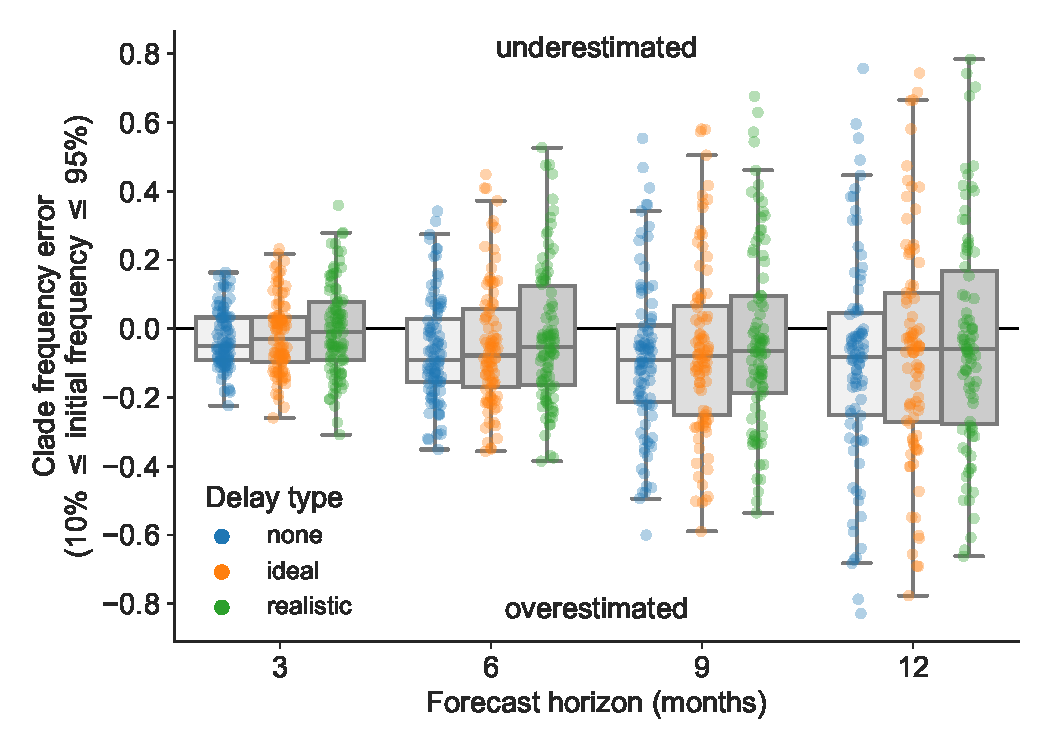
\includegraphics[width=\linewidth]{figures/h3n2_forecast_frequency_errors_by_delay_and_horizon}
\caption{Forecast clade frequency errors for natural H3N2 populations by forecast horizon in months and submission delay type (none, ideal, or observed).}
\label{fig:h3n2_forecast_clade_frequency_errors}
%
\figsupp[Absolute forecast clade frequency errors for H3N2 populations.]
{Absolute forecast clade frequency errors for natural H3N2 populations by forecast horizon in months and submission delay type (none, ideal, or observed).
  \figsuppdata{Current, estimated future, and observed future clade frequencies per initial timepoint, forecast horizon, and submission delay type for H3N2 populations; see \url{https://doi.org/xxx}}}
{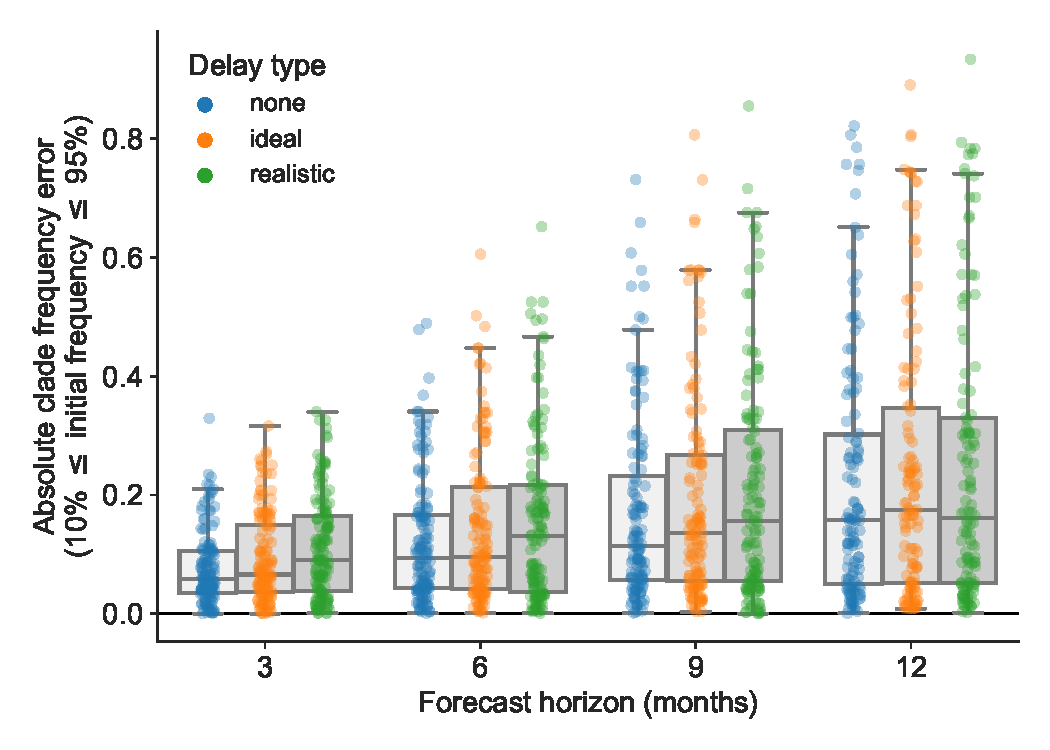
\includegraphics[width=6cm]{figures/h3n2_absolute_forecast_frequency_errors_by_delay_and_horizon}}\label{figsupp:h3n2_absolute_forecast_clade_frequency_errors}
%
\figsupp[Forecast clade frequency errors for simulated H3N2-like populations.]
{Forecast clade frequency errors for simulated H3N2-like HA populations by forecast horizon in months and submission delay type (none, ideal, or realistic).
  \figsuppdata{Current, estimated future, and observed future clade frequencies per initial timepoint, forecast horizon, and submission delay type for simulated H3N2-like populations; see \url{https://doi.org/xxx}}}
{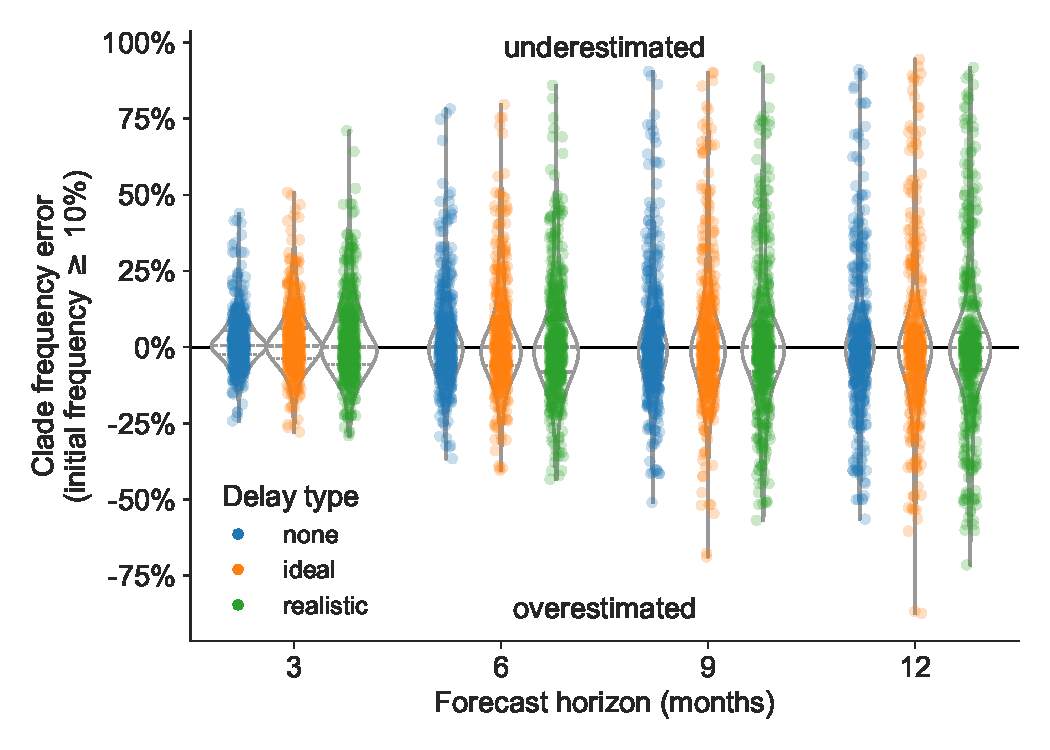
\includegraphics[width=6cm]{figures/simulated_forecast_frequency_errors_by_delay_and_horizon}}\label{figsupp:simulated_forecast_clade_frequency_errors}
%
\figsupp[Absolute forecast clade frequency errors for simulated H3N2-like populations.]
{Absolute forecast clade frequency errors for simulated H3N2-like HA populations by forecast horizon in months and submission delay type (none, ideal, or realistic).
  \figsuppdata{Current, estimated future, and observed future clade frequencies per initial timepoint, forecast horizon, and submission delay type for simulated H3N2-like HA populations; see \url{https://doi.org/xxx}}}
{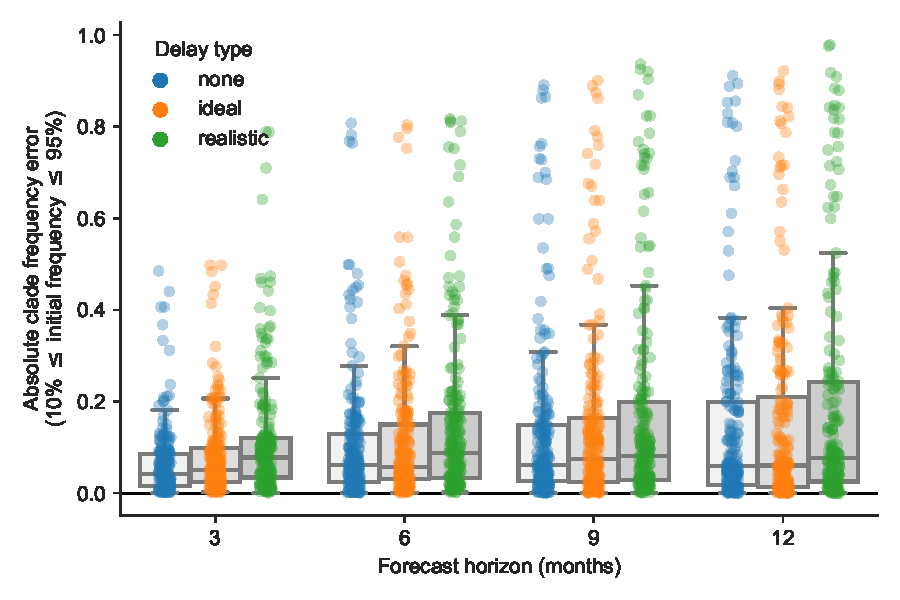
\includegraphics[width=6cm]{figures/simulated_absolute_forecast_frequency_errors_by_delay_and_horizon}}\label{figsupp:simulated_absolute_forecast_clade_frequency_errors}
%
\figdata{Current, estimated future, and observed future clade frequencies per initial timepoint, forecast horizon, and submission delay type for H3N2 populations.}\label{figdata:h3n2_clade_frequencies}
\figsrccode{Jupyter notebook used to produce this figure and the supplemental figures lives in \texttt{workflow/notebooks/plot-forecast-clade-frequency-errors-by-delay-type-and-horizon-for-population.py.ipynb}.}\label{figsrccode:forecast_clade_frequency_errors}
\end{figure}

\begin{table}[htb]
  \begin{center}
    
\begin{tabular*}{1.0\textwidth}{rrrrrrrrrr}
\toprule
        &            & \multicolumn{5}{c}{Clade frequency error (\%)} & \multicolumn{3}{c}{Absolute frequency error (\%)} \\
Horizon & Delay type & Mean & Median & Std Dev & Min & Max & Mean & Median & Std Dev \\
\midrule

3 & none & 1 & 0 & 9 & -28 & 28 & 7 & 6 & 6 \\
3 & ideal & 1 & 0 & 11 & -32 & 36 & 8 & 6 & 7 \\
3 & realistic & 1 & 0 & 13 & -31 & 50 & 10 & 7 & 9 \\
6 & none & 1 & 0 & 17 & -48 & 45 & 12 & 9 & 11 \\
6 & ideal & 1 & 0 & 19 & -50 & 53 & 13 & 9 & 13 \\
6 & realistic & 1 & 0 & 20 & -52 & 75 & 15 & 12 & 14 \\
9 & none & 0 & -1 & 23 & -66 & 59 & 16 & 10 & 17 \\
9 & ideal & 1 & -1 & 25 & -67 & 58 & 18 & 11 & 18 \\
9 & realistic & 1 & -1 & 26 & -67 & 79 & 19 & 12 & 19 \\
12 & none & 0 & 0 & 30 & -82 & 76 & 20 & 10 & 22 \\
12 & ideal & 1 & 0 & 31 & -80 & 74 & 21 & 9 & 23 \\
12 & realistic & 0 & 0 & 31 & -78 & 78 & 20 & 12 & 23 \\

\bottomrule
\end{tabular*}


    \caption{Errors in clade frequencies between observed and predicted values by forecast horizon (in months) and submission delay for H3N2 clades with an initial frequency $\geq$10\%.}
    \label{tab:h3n2_forecast_clade_frequency_errors}
  \end{center}
\end{table}

\begin{table}[htb]
  \begin{center}
    
\begin{tabular*}{0.7\textwidth}{rrrrr}
\toprule
        &            & \multicolumn{3}{c}{Absolute clade frequency error} \\
Horizon & Delay type & Mean & Median & Std Dev \\
\midrule

3 & none & 0.07 & 0.06 & 0.06 \\
6 & none & 0.13 & 0.09 & 0.11 \\
9 & none & 0.18 & 0.12 & 0.18 \\
12 & none & 0.23 & 0.13 & 0.24 \\
3 & ideal & 0.09 & 0.07 & 0.08 \\
6 & ideal & 0.15 & 0.11 & 0.14 \\
9 & ideal & 0.21 & 0.12 & 0.20 \\
12 & ideal & 0.25 & 0.15 & 0.26 \\
3 & realistic & 0.11 & 0.08 & 0.09 \\
6 & realistic & 0.17 & 0.12 & 0.15 \\
9 & realistic & 0.22 & 0.14 & 0.21 \\
12 & realistic & 0.25 & 0.14 & 0.27 \\

\bottomrule
\end{tabular*}


    \caption{Absolute errors in clade frequencies between observed and predicted values by forecast horizon (in months) and submission delay for H3N2 clades with an initial frequency $\geq$10\%.}
    \label{tab:h3n2_absolute_forecast_clade_frequency_errors}
  \end{center}
\end{table}

\subsection{Effects of realistic interventions on forecast accuracy}

Although we have investigated the effects of a range of forecast horizons and submission delays, not all of these scenarios are currently realistic.
The most we can hope to reduce the forecast horizon with current mRNA vaccine technology is from 12 months to 6 months and the most we could reduce submission delays would be from an average of 3 months to 1 month \citep{Grant2023}.
Additionally, we have not so far accounted for variation in populations per timepoint and clade when estimating the effects of these factors.
To determine the effects of realistic interventions on forecast accuracy, we therefore inspected the reduction in forecast error associated with improved vaccine development (reducing forecast horizon from 12 months to 6 months), improved genomic surveillance (reducing delays from current realistic to ideal), and the combination of both improvements.
We first selected all forecasts with a 12-month horizon and realistic delay for clades circulating at $\ge$10\% and $<$95\% frequency.
These forecasts represented the ``status quo''.
We then selected forecasts for the same future timepoints and clades for a 6-month horizon and realistic delay, 12-month horizon and ideal delay, and 6-month horizon and ideal delay.
We calculated the improvement in forecast accuracy as the difference in absolute forecast clade frequency error for a given future timepoint and clade between the status quo and each intervention.
Positive values represent improved forecast accuracy under a given intervention scenario and negative values represent a reduction in accuracy.

\begin{figure}[htb]
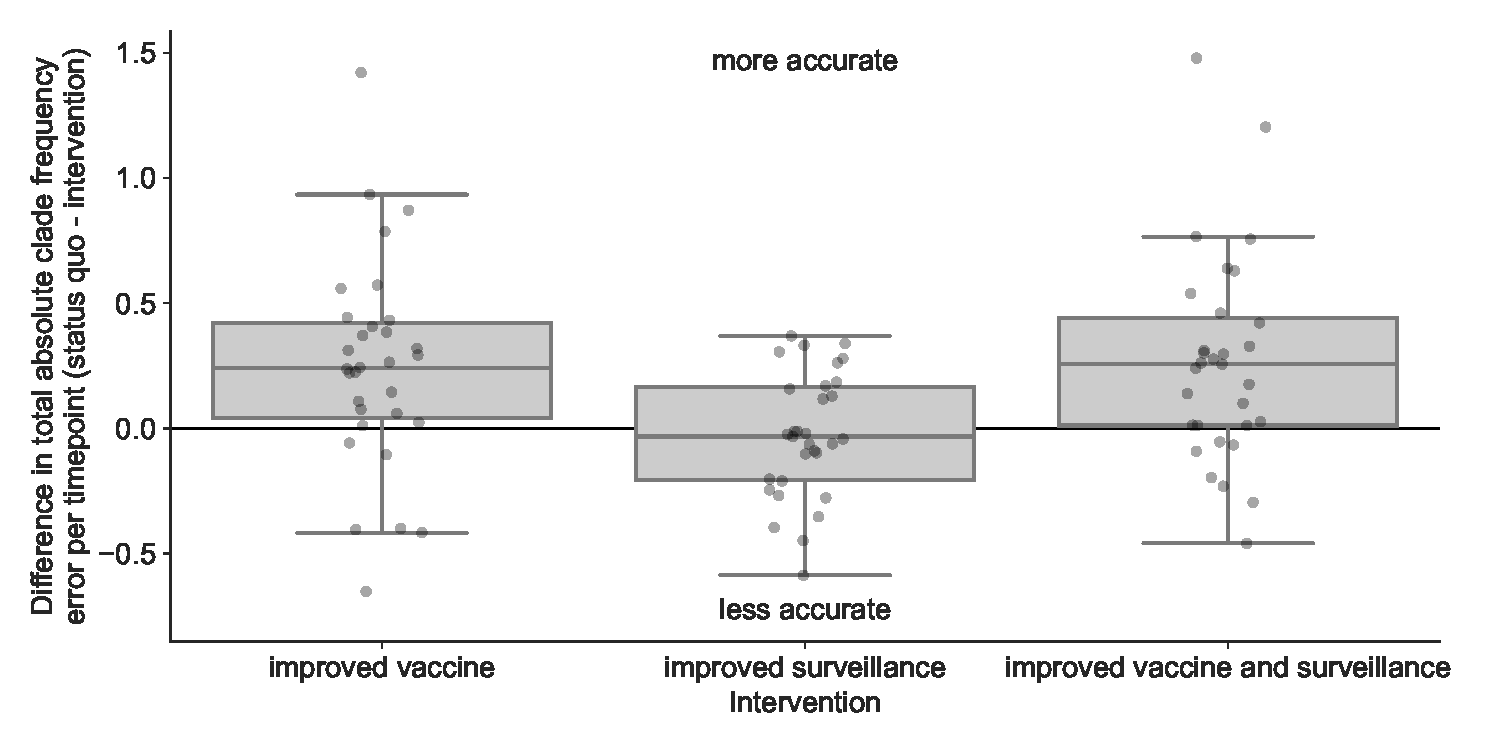
\includegraphics[width=\linewidth]{figures/h3n2_effects_of_realistic_interventions}
\caption{Improvement of clade frequency errors for H3N2 populations between the status quo and realistic interventions.}
\label{fig:h3n2_effects_of_realistic_interventions}
%
\figsupp[Improvement of clade frequency errors for simulated H3N2-like populations]
{Improvement of clade frequency errors for simulated H3N2-like populations between the status quo and realistic interventions.
  \figsuppdata{Differences in absolute clade frequency error per future timepoint and clade between the status quo and realistic interventions for simulated H3N2-like populations; see \url{https://doi.org/xxx}}}
{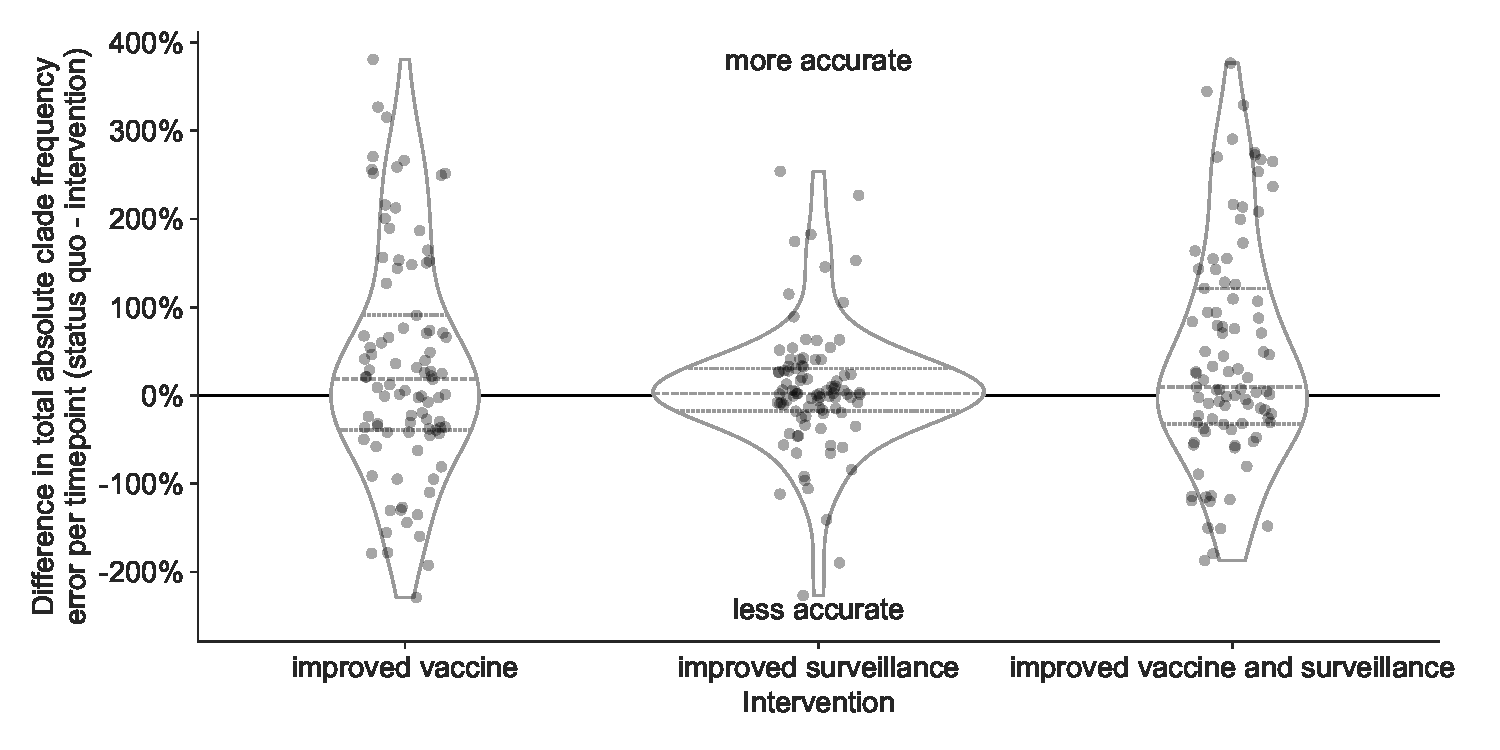
\includegraphics[width=6cm]{figures/simulated_effects_of_realistic_interventions}}\label{figsupp:simulated_effects_of_realistic_interventions}
%
\figdata{Differences in absolute clade frequency error per future timepoint and clade between the status quo and realistic interventions for H3N2 populations.}\label{figdata:h3n2_effects_of_realistic_interventions}
\figsrccode{Jupyter notebook used to produce this figure and the supplemental figure lives in \texttt{workflow/notebooks/plot-forecast-clade-frequency-errors-by-delay-type-and-horizon-for-population.py.ipynb}.}\label{figsrccode:effects_of_realistic_interventions}
\end{figure}

\begin{table}[htb]
  \begin{center}
    
\begin{tabular*}{1.0\textwidth}{rrrrrr}
\toprule
             & \multicolumn{3}{c}{Forecast accuracy improvement (\%)} & \multicolumn{2}{c}{Forecasts improved} \\
Intervention & Mean & Median & Std Dev & Total & Proportion \\
\midrule

improved vaccine & 32 & 33 & 46 & 23 & 0.74 \\
improved surveillance & -6 & -1 & 24 & 13 & 0.42 \\
improved vaccine and surveillance & 33 & 42 & 45 & 24 & 0.77 \\

\bottomrule
\end{tabular*}


    \caption{Improvement in H3N2 forecasts under realistic interventions of improved vaccine development (reducing 12-month to 6-month forecast horizon), improved surveillance (reducing submission delays from 3 months on average to 1 month), or a combination of both interventions.
      We measured improvements from the status quo (12-month forecast horizon and 3-month average submission delay) for clades with an initial frequency of $\geq$10\% as the difference in absolute clade frequency error per future timepoint and clade and the number and proportion of future timepoint and clade forecasts that improved under the intervention.}
    \label{tab:h3n2_effects_of_realistic_interventions}
  \end{center}
\end{table}

\section{Discussion}

TKTK

\section{Methods and Materials}

\subsection{Estimating and assigning submission delays}

We estimated the delay between sample collection and submission of A/H3N2 hemagglutinin (HA) sequences to the GISAID database \citep{gisaid} by calculating the difference in GISAID-annotated submission date and collection date in days for samples collected between January 1, 2019 and January 1, 2020 and with a submission date prior to October 1, 2020.
We selected this period of time as representative of modern genomic surveillance efforts prior to changes in circulation patterns of influenza caused by the SARS-CoV-2 pandemic.
Of the 104,392 HA sequences in GISAID, 11,222 (11\%) were collected during this period with a mean submission delay of 98 days ($\sim$3 months) and a median delay of 74 days.
Only 11\% of sequences (N=1,210) were submitted within 4 weeks of collection, and only 36\% (N=4,057) were submitted within 8 weeks (\FIG{model_of_delays_and_horizons}A, purple).

We modeled the shape of the observed delay distribution as a gamma distribution using a maximum likelihood fit from SciPy 1.10.1 \citep{scipy}.
With this approach, we estimated a shape parameter of 1.76, a scale parameter of 53.18, and location parameter of 3.98.
The product of these shape and scale values corresponded to a mean delay of 93.76 days (\FIG{model_of_delays_and_horizons}A, green).
To assign realistic submission delays to each sample in our analysis, we randomly sampled from this gamma distribution and calculated a ``realistic submission date'' by adding the sampled delay in days to the observed collection date.

Based on the observed rapid submission of SARS-CoV-2 genomes during the first years of the pandemic, we expected that an achievable ``ideal'' submission delay for seasonal influenza sequences would have a 1-month average delay instead of the observed $\sim$3-month delay from the pre-pandemic period.
We modeled this ideal submission delay distribution by dividing the gamma shape parameter by 3 to get a value of 0.59 and a corresponding mean delay of 31.25 days (\FIG{model_of_delays_and_horizons}A, orange).
This approach effectively shifted the realistic gamma toward zero, while maintaining the relatively longer upper tail of the distribution.
To assign ideal submission delays to each sample in our analysis, we randomly sampled from this modified gamma distribution and added the sampled delay in days to the observed collection date.
Additionally, we required that each sample's ``ideal'' delay be less than or equal to its ``realistic'' delay.

\subsection{Forecasting with different forecast horizons}

We tested the effect of forecasting future influenza populations at forecast horizons of 3, 6, 9, and 12 months (\FIG{model_of_delays_and_horizons}B).
Previously, we produced forecasts every 6 months starting from October 1 and April 1 and predicting 12 months into the future \citep{Huddleston2020}.
To support forecasts in 3-month intervals, we produced annotated time trees for 6 years of HA sequences every 3 months with data available up to the first day of January, April, July, and October.
We produced these trees for each timepoint with three different delay scenarios: no delay, ideal delay, and realistic delay.
For each scenario, we selected sequences for analysis at a given timepoint based on their collection date, ideal submission date, or realistic submission date, respectively.
This experimental design produced forecasts for three delay types at each of the four forecast horizons (e.g., \FIG{model_of_delays_and_horizons}B, blue, green, and orange initial timepoints for the 3-month forecast horizon).

Since submission dates were not available prior to April 2005, our analysis of natural A/H3N2 sequences spanned from April 1, 2005 to October 1, 2019.
To simplify the data required for these analyses, we produced forecasts of natural A/H3N2 populations with our best sequence-only model from our prior work \citep{Huddleston2020}, a composite model based on local branching index (LBI) \citep{Neher:2014eu} and mutational load \citep{Luksza:2014hj}.
For simulated A/H3N2-like populations, we produced forecasts with the ``true fitness'' model that relies on the normalized fitness value of each simulated sample.

Each forecast generated a predicted future frequency per sequence in the initial timepoint's tree.
As in our prior work, we calculated the earth mover's distance \citep{Rubner1998} between the predicted and observed future populations using HA amino acid sequences from initial and future timepoints, predicted future frequencies from the initial timepoint, and observed future frequencies from future timepoint.
For the future timepoint, we used data from the ``no delay'' scenario as our truth set, regardless of the delay scenario for the initial timepoint.
This design allowed us to measure the effect of ideal and realistic submission delays on forecast accuracy relative to a scenario with no delays.

\subsection{Defining clades}

Official clade definitions do not exist for all time periods of our analysis of A/H3N2 populations and do not exist at all for simulated A/H3N2-like populations.
Therefore, we defined ``clades'' for natural and simulated HA trees based on the amino acid haplotypes of HA at 49 previously defined epitope sites \citep{Luksza:2014hj}.
This definition of clades follows from realistic clade definitions that tend to depend on mutations in HA1 at known epitope sites.
Although this automated haplotype-based definition of clades tended to create monophyletic groups, the same haplotype could emerge multiple times independently in different phylogenetic clades.

For each tree in our analysis, we assigned clade labels to each tip and internal node based on their amino acid haplotype at epitope sites.
For each tip, this clade label was deterministic across trees, as the sequence of a tip did not change.
Tips also inherited the clade labels of their ancestral nodes in the tree, allowing us to estimate frequencies of larger clades based on the frequencies of tips in those clades.
However, the inferred sequence at internal nodes varied with the tips present in a given tree.
For example, submission delays could change the tips present in trees representing the same timepoint, resulting in different internal nodes and inferred sequences.
Additionally, the continued accumulation of amino acid mutations between timepoints changed the composition of internal nodes over time, complicating the comparison of large clades between initial and future timepoints of a forecast.

To stably define clades for internal nodes in our analysis, we created a single tree with all HA sequences present in our analysis and without delayed sequence submission.
We inferred ancestral sequences for internal nodes in this tree and assigned clades to each node and tip based on their amino acid haplotypes.
We created a mapping between each tip and the clades it descended from that allowed us to track clade frequencies across 6-year trees built per timepoint in the analysis.

\subsection{Estimating current and future clade frequencies}

We estimated current clade frequencies for each timepoint in our analysis by summing the frequencies of tips in a given timepoint's tree by the clade assigned to each tip.
To inspect the effects of submission delays on clade frequency estimates, we calculated the clade frequency error per timepoint and clade by subtracting the clade frequency estimated with ideal or realistic delayed sequence submission from the corresponding clade frequency without delays.
We compared the effects of submission delays for clades of different sizes by filtering clades by their frequency estimated without delays to small clades ($\ge$1\% and $<$10\%) and large clades ($\ge$10\%).

We estimated future clade frequencies for each combination of delay type, initial timepoint, and future timepoint in the analysis using the following steps.
First, we merged the frequencies per tip at each timepoint with all forecasts from the same timepoint.
The resulting table included the initial and predicted frequencies for each tip for each combination of initial timepoint, forecast horizon, and submission delay.
To define the observed future population for each forecast, we selected all tips that were present in the future timepoint of the corresponding dataset without submission delays.
Using the tip-to-clade mapping described above, we found all clades that were present at both initial and future timepoints.
We calculated the initial and predicted future frequencies per clade at the initial timepoint by summing the frequencies of all tips in each clade.
We calculated the observed future frequencies per clade at the future timepoint with the same approach.
Finally, we merged the initial and predicted future frequencies with the observed future frequencies by clade, keeping all clades that were present in the initial timepoint.
To focus our analysis on the most biologically relevant clades, we limited our analysis to clades that had an initial frequency $\ge$10\% and $\le$95\% under the scenario with no delay.

\section{Acknowledgments}

TKTK

\nocite{*} % This command displays all refs in the bib file. PLEASE DELETE IT BEFORE YOU SUBMIT YOUR MANUSCRIPT!
\bibliography{delays}

\end{document}
